\documentclass[10pt, letterpaper]{article}
\usepackage{geometry}
\geometry{
 a4paper,
 total={170mm,257mm},
 left=20mm,
 top=20mm,
 }
\usepackage{graphicx} % Required for inserting images
\usepackage[english,greek]{babel}
\usepackage{amsmath} 
\usepackage{subcaption}
\usepackage{dirtytalk}
\usepackage{hyperref}
\usepackage{comment}
\usepackage{tikz}
\usepackage{caption}
\usepackage{float}
\usepackage{amssymb}
\usepackage{indentfirst}
\newcommand{\en}{\selectlanguage{english}}
\newcommand{\gr}{\selectlanguage{greek}}


\graphicspath{{../plots/}} % specify the path to the images

\title{Εργασία Υπολογιστικού Ηλεκτρομαγνητισμού}
\author{Φίλιππος Ρωσσίδης \\ (ΑΕΜ 10379)}
\date{\today}


\begin{document}
\maketitle


\section*{Μέρος Α}

Στο πρώτο μέρος της εργασίας θα χρησιμοποιήσουμε την μέθοδο \en FEM \gr για να επιλύσουμε δύο ηλεκτροστατικά προβλήματα: ενός ομοαξονικού καλωδίου 
(σχήμα \ref{fig:coaxial}) όπου ο εσωτερικός αγωγός τίθεται σε δυναμικό 1 \en Volt \gr και ο εξωτερικός σε 0 \en Volt, \gr 
και ενός πυκνωτή απείρου μήκους, με διαστάσεις που φαίνονται στο σχήμα \ref{fig:capacitor} και διαφορά δυναμικού \en V. \gr

Θα χρησιμοποιήσουμε την μέθοδο \en FEM \gr για την εύρεση του δυναμικού στο χώρο και έπειτα απο το δυναμικό θα υπολογίσουμε 
το ηλεκτρικό πεδίο, την ενέργεια και την χωρητικότητα. 


\begin{figure}[H]
    \centering
    % Subfigure (a): Ομοαξονικό
    \begin{subfigure}[b]{0.45\textwidth}
      \centering
      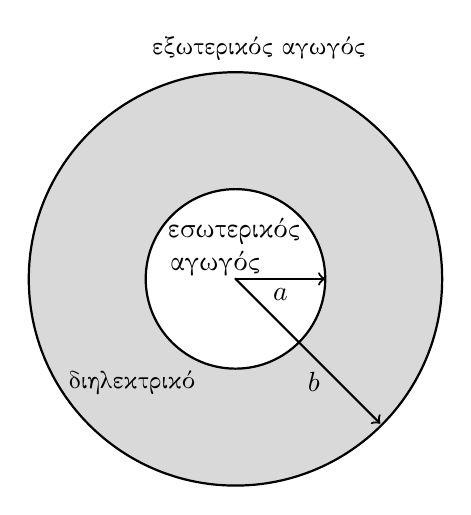
\begin{tikzpicture}[scale=1.5]
        % Radii
        \def\a{0.76}
        \def\b{1.75}
      
        % Annular dielectric region (from a to b)
        \fill[gray!30] (0,0) circle (\b);
        \fill[white] (0,0) circle (\a); % Inner conductor kept white
      
        % Outer conductor
        \draw[thick] (0,0) circle (\b);
      
        % Inner conductor (white-filled with border)
        \draw[thick] (0,0) circle (\a);
      
        % Radius a (along x-axis)
        \draw[->, thick] (0,0) -- (\a,0);
        \node[below] at (\a/2, 0) {\( a \)};
      
        % Radius b (along diagonal)
        \draw[->, thick] (0,0) -- (1.4 /2 * \b ,- 1.4 / 2* \b);
        \node[left] at (\b/2.2, -\b/2) {\( b \)};
      
        % Center point
        \fill (0,0) circle (0.01);
      
        % Labels
        \node[align=center, text width=1.2cm] at (-0.17, \a - 0.5) {εσωτερικός\\αγωγός};
        \node at (0.2, \b + 0.2) {\small εξωτερικός αγωγός};
        \node at (-\b/2, -\b/2) {\small διηλεκτρικό};
      \end{tikzpicture}
      \caption{Ομοαξονικό καλώδιο}
      \label{fig:coaxial}
    \end{subfigure}
    \hfill
    % Subfigure (b): Πυκνωτής
    \begin{subfigure}[b]{0.45\textwidth}
        \centering
        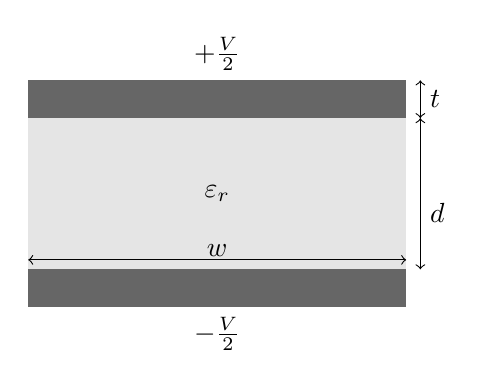
\begin{tikzpicture}[scale=1.2]
        \def\d{2}   % Απόσταση μεταξύ πλακών
        \def\w{4}   % Πλάτος πλακών
        \def\t{0.4}   % Πάχος πλακών
    
        % Κάτω πλάκα (με λίγο κενό κάτω για να χωρέσει η διάσταση w)
        \fill[black!60] (-\w/2, 0.3) rectangle (\w/2, 0.3+\t);
        \node[below] at (0, 0.3) {\( -\frac{V}{2} \)};
    
        % Πάνω πλάκα
        \fill[black!60] (-\w/2, 0.3+\d) rectangle (\w/2, 0.3+\d+\t);
        \node[above] at (0, 0.3+\d+\t) {\( +\frac{V}{2} \)};
    
        % Διηλεκτρικό
        \fill[gray!20] (-\w/2, 0.3+\t) rectangle (\w/2, 0.3+\d);
    
        % Διαστάσεις
        % Απόσταση d
        \draw[<->] (\w/2 + 0.15, 0.3+\t) -- (\w/2 + 0.15, 0.3+\d);
        \node[right] at (\w/2 + 0.15, 0.3+\d/2) {\( d \)};
        
        % Πλάτος w
        \draw[<->] (-\w/2, 2* \t) -- (\w/2, 2 * \t);
        \node at (0, 2 * \t + 0.1) {\( w \)};
    
        % Πάχος t (πάνω πλάκας)
        \draw[<->] (\w/2 + 0.15, 0.3+\d) -- (\w/2 + 0.15, 0.3+\d+\t);
        \node[right] at (\w/2 + 0.15, 0.3+\d+\t/2) {\( t \)};
    
        % Διηλεκτρική σταθερά στο κέντρο
        \node at (0, 0.5+\d/2) {\( \varepsilon_r \)};
        \end{tikzpicture}
        \caption{Πυκνωτής επίπεδων πλακών}
        \label{fig:capacitor}
    \end{subfigure}
    \caption{}
    \label{fig:definition}
  \end{figure}


\subsection*{Σύντομη περιγραφή της μεθόδου \en FEM \gr για την εύρεση δυναμικού σε ηλεκτροστατικό πρόβλημα}

Θα παρουσιάσω σύντομα την μέθοδο, για την πληρότητα της αναφοράς. Σε κάποια σημεία χρησιμοποιώ διαφορετικό 
συμβολισμό από τις σημειώσεις γιατι το θεώρησα πιο ευανάγνωστο.

Αρχικά, εφόσον λύνουμε δισδιάστατα προβλήματα, χωρίζουμε τον υπολογιστικό χώρο σε \en 2d simplexes \gr δηλαδή τρίγωνα. 
Αν οριστούν οι συντεταγμένες \en simplex \gr ενός σημείου $(x,y)$ ως $\zeta_i(x,y) = h_i / H_i$ όπου $h_i$ η απόσταση του σημείου 
από την πλευρά που δεν περιέχει τον κόμβο $i$ και $H_i$ το ύψος από τον κόμβο $i$, τότε 
\[ \zeta_i(x,y) = a_i + b_ix + c_iy, \ \ i = 1,2,3 \]
όπου τα $a_i,b_i,c_i$ δίνονται με κυκλική εναλλαγή απο τις:
\begin{equation} \label{eq:abc}
  a_1 = \frac{x_2 y_3 - x_3 y_2}{D}, \quad
b_1 = \frac{y_2 - y_3}{D}, \quad
c_1 = \frac{x_3 - x_2}{D},
\end{equation}
\[ D =  
\left| 
\begin{array}{@{}ccc@{}}
1 & x_1 & y_1 \\
1 & x_2 & y_2 \\
1 & x_3 & y_3 \\
\end{array} 
\right|
\]
Αναλύουμε, εντός του τριγώνου, το δυναμικό ως 
\[ \phi \approx \sum_{i=1}^3 \phi_iN_i^t\]
όπου $\phi_i$ το δυναμικό στον κόμβο $i$ και διαλέγουμε $N_i^t=\zeta_i$ τις τοπικές (εντός του τριγώνου $t$) συναρτήσεις βάσης.
Σκοπός μας είναι να βρούμε τις κατάλληλες τιμές $\phi_i$ για κάθε κόμβο στον υπολογιστικό χώρο.
Έτσι ορίζουμε τις ολικές συναρτήσεις βάσης ως 
\[ N_p = \sum_{t | p \in t} N_i^t \]
όπου $t$ τρίγωνο τέτοιο ώστε ο κόμβος $p$ να ανήκει σε αυτό, και $i$ η τοπική αρίθμηση του $p$ στο $t$.
Το δυναμικό αναλύεται συνολικά:
\begin{equation} \label{eq:phi_approx}
  \phi \approx \sum_{p=1}^{N_n} \phi_pN_p
\end{equation}
όπου $N_n$ το πλήθος κόμβων.
Θα λύσουμε την εξίσωση \en Poisson: \gr 
\[ \nabla \cdot (\epsilon \nabla \phi) + \rho = 0\]
χρησιμοποιώντας την μέθοδο \en Galerkin \gr η οποία αποτελεί κατηγορία της μεθόδου σταθμισμένων υπολοίπων:
\[ \langle \phi', \nabla \cdot (\epsilon \nabla \phi) + \rho \rangle = 0 \]
όπου διαλέγουμε ως συναρτήσεις 
δοκιμής $\phi'$ τις συναρτήσεις βάσης $N_i$, οπότε:
\[ \iint_{\Omega} \phi' [ \nabla \cdot (\epsilon \nabla \phi) + \rho ] ds = 0, \ \ \forall \phi' \in \{N_i\} \]
όπου $\Omega$ ο υπολογιστικός χώρος. 
Οι παραπάνω είναι τόσες εξισώσεις όσους έχουμε αγνώστους κόμβους, τους οποίους θα βρούμε λύνοντας το σύστημα.
Ισοδύναμα γράφονται:
\begin{equation} \label{eq:weak_form}
  -\iint_{\Omega} \nabla \phi' \cdot \epsilon \nabla \phi ds +  \oint_{c} \phi' \epsilon \frac{\partial \phi}{\partial \hat{n}}dl + \iint_{\Omega} \phi' \rho ds = 0
\end{equation}
όπου $c$ το όριο της επιφάνειας $\Omega$. Επειδή έχουμε είτε συνθήκες \en Dirichlet \gr (γνωστό $\phi$)  είτε \en Neumann \gr 
($\frac{\partial \phi}{\partial \hat{n}} = 0$) στο όριο, ο δεύτερος όρος της εξίσωσης (\ref{eq:weak_form}) ισούται με 0. Επίσης και στα δύο προβλήματα 
δεν υπάρχουν φορτία ($\rho = 0$), άρα:
\[ \iint_{\Omega} \nabla \phi' \cdot \epsilon \nabla \phi ds = 0\]
Διακριτοποιώ αντικαθιστώντας την εξίσωση (\ref{eq:phi_approx}), επίσης αφού $\phi' \in \{N_i\}$ γράφω στη θέση του $N_q$ για κάποιο $q \in \{1,..,N_n\}$:
\[ \iint_{\Omega} \nabla N_q(\mathbf{r}) \cdot \epsilon \nabla (\sum_p \phi_p N_p(\mathbf{r}))  ds = 0 \Rightarrow\]
\begin{equation} \label{eq:sum_out}
  \sum_p \epsilon \phi_p \iint_{\Omega} \nabla N_q(\mathbf{r}) \cdot \nabla N_p(\mathbf{r})ds = 0
\end{equation}

Ισχύει:
\[ N_i^t (x,y) =  \zeta_i(x,y) = a_i + b_ix + c_iy, \text{\ εντός του στοιχείου και $0$ αλλού}\Rightarrow\]
\[ \nabla N_i^t =   
    \begin{bmatrix}
        b_i \\
        c_i
    \end{bmatrix}
                    , \text{\ εντός του στοιχείου και $0$ αλλού}\]
Για κάθε κόμβο η ολική συνάρτηση βάσης εντός κάθε τριγώνου στο οποίο αυτός ανήκει ισούται με 
την τοπική συνάρτηση βάσης του και εκτός αυτών με μηδέν.
Έπεται ότι το γινόμενο $\nabla N_p \cdot \nabla N_q$ ισούται με $0$ για μη γειτονικούς κόμβους. Για γειτονικούς κόμβους $p,q$ όπου 
ανήκουν και οι δύο σε κάποιο 
τρίγωνο $t$, ισχύει εντός του τριγώνου
\[ \nabla N_p  \cdot \nabla N_q  = \nabla N_i^t \cdot \nabla N_j^t = 
    \begin{bmatrix}
        b_i \\
        c_i
    \end{bmatrix}
      \cdot 
    \begin{bmatrix}
        b_j \\
        c_j        
    \end{bmatrix}
    =  b_ib_j + c_ic_j
\]
με $i,j$ την τοπική αρίθμηση εντός του $t$. Έτσι:
\begin{equation} \label{eq:int_of_grad_Np_Nq_}
  \iint_S \nabla N_p  \cdot \nabla N_q  dS = \sum_{t | p,q \in t} (b_ib_j + c_ic_j) A_e 
\end{equation}
όπου $i,j$ η τοπική αρίθμηση των κόμβων $p,q$ στο τρίγωνο $t$, οι $b,c$ δίνονται από την (\ref{eq:abc}) και $A_e = D/2$ το εμβαδόν του τριγώνου.
Η (\ref{eq:sum_out}) γράφεται:
\begin{equation}  \label{eq:system_non_matrix_form}
  \sum_p \epsilon \phi_p \sum_{t | p,q \in t} (b_ib_j + c_ic_j) A_e  = 0   \ \ \forall q \in \{1,..,N_n\}
\end{equation}
Αν ορίσω τον τετραγωνικό πίνακα $N_n \times N_n$ $\mathbf{S}$:
\[ \mathbf{S}[p,q] = \epsilon \sum_{t | p,q \in t} (b_ib_j + c_ic_j) A_e  \]
και τον πίνακα στήλη $1 \times N_n$ $\mathbf{F}$ που περιέχει τα δυναμικά των κόμβων $\phi_p$, τότε το σύστημα (\ref{eq:system_non_matrix_form}) γράφεται:
\[ \mathbf{S} \cdot \mathbf{F} = 0 \]

Μπορούμε να υπολογίσουμε εύκολα τον πίνακα $\mathbf{S}$ αν απαριθμήσουμε κάθε τρίγωνο στον χώρο και έπειτα για κάθε έναν από τους
9 συνδυασμούς των κόμβων του (έστω $p,q$ ολικά, $i,j$ τοπικά) υπολογίσουμε την ποσότητα $\epsilon (b_ib_j + c_ic_j) A_e$ και την προσθέσουμε στην θέση $[p,q]$ του πίνακα.

Τέλος πρέπει να υπολογίσουμε τους κόμβους με οριακή συνθήκη \en Dirichlet \gr δηλαδή γνωστούς. Επειδή ο πίνακας $\mathbf{F}$ είναι η λύση,
δεν μπορεί να περιλαμβάνει τα γνωστά δυναμικά, έτσι τον χωρίζουμε τοποθετώντας πρώτα τα άγνωστα και έπειτα τα γνωστά:

\[
\mathbf{F} = 
\left[ \begin{array}{@{}c@{}}
\mathbf{F}_f \\
\hline
\mathbf{F}_p
\end{array} \right]
, \ \
\mathbf{S} = 
\left[ \begin{array}{@{}c|c@{}}
  \mathbf{S}_{ff} & \mathbf{S}_{fp} \\
  \hline
  \mathbf{S}_{pf} & \mathbf{S}_{pp}
  \end{array} \right]
\]
Τότε:
\begin{equation}   \label{eq:FEM}
  \mathbf{S}_{ff} \cdot \mathbf{F}_f = - \mathbf{S}_{fp} \cdot \mathbf{F}_p
\end{equation}

Λύνοντας το σύστημα (\ref{eq:FEM}) ως προς $\mathbf{F}_f$ βρίσκουμε τα άγνωστα δυναμικά σε κάθε κόμβο του χώρου.




\subsubsection*{Αλγόριθμος ενέργειας}

Αφού έχουμε βρει το δυναμικό σε κάθε κόμβο, θα υπολογίσουμε την συνολική ενέργεια ανά μονάδα μήκους:


\[W_e = \frac{1}{2} \iint_S \epsilon |\mathbf{E}|^2dS = \frac{1}{2} \iint_S \epsilon \nabla \phi  \cdot \nabla \phi dS\]
αναλύω το δυναμικό στις συναρτήσεις βάσης σύμφωνα με την (\ref{eq:phi_approx}):
\[W_e \approx \frac{1}{2} \iint_S \epsilon \nabla (\sum_p \phi_p N_p(\mathbf{r}))  \cdot \nabla (\sum_q \phi_q N_q(\mathbf{r})) dS\]
γνωρίζουμε τις τιμές $\phi_p$, το $\epsilon$ είναι σταθερό στον χώρο και τα αθροίσματα είναι πεπερασμένα, οπότε:
\[ W_e \approx  \frac{1}{2} \epsilon \iint_S  \sum_p \{ \phi_p \nabla N_p(\mathbf{r}) \} \cdot  \sum_q \{ \phi_q \nabla N_q(\mathbf{r}) \} dS\]
\[ = \frac{1}{2} \epsilon  \sum_p \sum_q  \phi_p \phi_q \iint_S \nabla N_p(\mathbf{r})  \cdot \nabla N_q(\mathbf{r})  dS \]
Αν συμβολίσω $N_i^t$ τις \emph{τοπικές} συναρτήσεις βάσης του κόμβου $i$ ενός τριγώνου $t$, για τριγωνικά στοιχεία πρώτης τάξης ισχύει: 
\[ N_i^t (x,y) =  \zeta_i(x,y) = a_i + b_ix + c_iy, \text{\ εντός του στοιχείου και $0$ αλλού}\Rightarrow\]
\[ \nabla N_i^t =   
    \begin{bmatrix}
        b_i \\
        c_i
    \end{bmatrix}
                    , \text{\ εντός του στοιχείου και $0$ αλλού}\]
Αντικαθιστώντας από την (\ref{eq:int_of_grad_Np_Nq_}):
\[ W_e \approx \frac{1}{2} \epsilon  \sum_p \sum_{q \in N(p)}  \phi_p \phi_q   \sum_{t | p,q \in t} (b_i^tb_j^t + c_i^tc_j^t) A_e^t  \]
\[ =   \sum_p \sum_{q \in N(p)} \frac{1}{2} \epsilon  \phi_p \phi_q   \sum_{t | p,q \in t} (b_i^tb_j^t + c_i^tc_j^t) A_e^t   \]
όπου ως $N(p)$ συμβολίζω τους γείτονες του κόμβου $p$ (συμπεριλαμβανομένου και του εαυτού του).

Για να γλυτώσουμε υπολογιστικό χρόνο μπορούμε, όπως και στον υπολογισμό του πίνακα $\mathbf{S}$, να απαριθμήσουμε όλα τα 
τρίγωνα και για κάθε έναν από τους $9$ συνδυασμούς των κόμβων να υπολογίζουμε την ποσότητα 
\[ \frac{1}{2} \epsilon  \phi_i \phi_j  (b_ib_j + c_ic_j) A_e   \]
και να την προσθέτουμε διαδοχικά στο αποτέλεσμα. 












\subsection*{Ομοαξονικό καλώδιο}

Το ομοαξονικό καλώδιο του σχήματος \ref{fig:coaxial} με $2b = 3.5 mm $ έχει χαρακτηριστική αντίσταση $50 \Omega$ και διηλεκτρικό 
τον αέρα. Ο εσωτερικός αγωγός τίθεται σε δυναμικό \en $\phi = 1 \ \text{Volt}$ \gr και ο εξωτερικός σε $\phi = 0$.

\subsubsection*{Υπολογισμός του α}


Η χαρακτηριστική αντίσταση ομοαξονική γραμμής μεταφοράς δίνεται από την:\footnote{Θεόδωρος Τσιμπούκης, Ηλεκτρομαγνητικό πεδίο, σελ. 933}
\[ Z_0 = \frac{1}{2 \pi}\sqrt{\frac{\mu}{\epsilon}} \ln (\frac{b}{a})  \]
Λύνοντας ως προς $a$
\[ a = b e^{-2\pi Z_0 \sqrt{\frac{\epsilon}{\mu}}}  = 1.75 \cdot 10^{-3} e^{-2\pi 50 \sqrt{\frac{\epsilon_0}{\mu_0}}}\]
Προκύπτει
\[a = 0.76 mm\]



\subsubsection*{Χωρητικότητα ομοαξονικού αναλυτικά }

Η ανά μονάδα μήκους χωρητικότητα κυλινδρικού πυκνωτή δίνεται από την:\footnote{Θεόδωρος Τσιμπούκης, Ηλεκτρομαγνητικό πεδίο, σελ. 145}
\[ C = \frac{2 \pi \epsilon}{\ln (\frac{b}{a})} =  6.67 \cdot 10^{-11} F\]

\subsubsection*{Κώδικας \en matlab \gr}

...

\subsubsection*{Αποτελέσματα}

...

\subsection*{Πυκνωτής}
\subsubsection*{Χωρητικότητα ανά μονάδα μήκους πυκνωτή}


\end{document}